\section{Numerical Model}
\label{sec:numerical_model}
\textit{This chapter will discuss the assumptions made in the development of the numerical model as well as the approach taken to calculate the internal stresses of the aileron.\\
Firstly the assumptions and idealisations are listed along with their arguments and significance. Secondly, the method that is used to make the simulation is explained. Furthermore, the load case and the governing equations of the numerical model are explained.}

\subsection{Assumptions and idealisations}
\label{subsec:assumptions_numerical}
The structure is idealised as a boom skin multi-cell beam structure. This assumption is reasonable, as the thickness of the skin is magnitudes smaller than the size of the structure, as well as the Moment of Inertia of a stringer is magnitudes smaller than its contribution to the bending stiffness by the parallel axis theorem. With this idealisation it is assumed that only the stiffeners carry normal stresses, while the skin only carries shear. Furthermore it is assumed that the material is behaving linearly in all load cases, this is a reasonable assumption if the maximum stress in the aileron stays below the yield stress of the material used.\\

\noindent As the structure is assumed to be thin walled with stringers in the direction of the x axis, compressive and tensile forces are only taken into account for this direction, as there are however no external forces acting in the x axis, the structure is assumed to be only in shear, bending, and torsion. These 3 can occur around all axes. However, bending around the y axis is neglected, as all 3 hinges are fixed in this direction and the moment of inertia for this bending is bigger than for the other directions while the forces causing it are smaller. Bending around the x axis is also neglected as the chord of the aileron is much shorter than the width of the aileron. Torsion is only considered around the x axis of the aileron as this direction has the smallest cross-section of the 3 possible cutting planes. Furthermore, shear in the x direction is not calculated, as it can be seen by inspection that no external forces are acting in the x axis. In addition, the weight of the aileron is neglected in all calculations. It is also assumed that the deformation of the aileron has no effect on the deformation of the wing.

\subsection{Load case decomposition}
\label{subsec:load_decomposition}
In the concerning loading scenario, two loads are present along with the bending of the aileron. These together cause reaction forces which cause deflection, twist of the structure and stresses in the structure. Instead of analysing the effects of the bending and the two loads simultaneously, the effects of multiple load cases are analysed separately. Afterwards these are added up to get to the total load decomposition. Three load cases are used in the model.

\subsubsection{First load case}
\noindent Firstly there is the deformation of the aileron, due to the wing-flex of the main wing. This deformation is described as bending around the z-axis. Naturally this causes a bending moment around the z-axis. Furthermore this causes reaction forces to appear in hinge 1 and 3 in the y-direction.\\

\noindent The aileron deformation is numerically interpolated using a natural cubic spline with three knots consisting of hinge 1, 2 and 3. Consequently there are two spline segments.

\subsubsection{Second load case}
\noindent The second load case consists of the aerodynamic load acting on the aileron. This is a non uniformly distributed load, varying in x- and z- direction and acting in negative y-direction. It introduces a bending moment around the x- and z- axis. Furthermore it causes torsion around the x-axis, due to its uneven distribution of the load itself. Finally there is also a shear stress in the y-direction. \\

\noindent The input data consists of values of the aerodynamic load along the aileron in x- and z-direction. Firstly this data is interpolated with the use of tensor product interpolation. Finally Gauss quadrature is used for 2D integration.

\subsubsection{Third load case}
\noindent The third and final load case that is being considered is the load acting on actuator II. This load causes bending around the z-axis and torsion around the x-axis. Furthermore, shear stress is introduced in the z- and y-axis.

\noindent For all these load cases the reaction forces can be calculated by setting a force and moment equilibrium.

\subsubsection{Decomposition}
\noindent When all of the loads acting on the aileron are known, normal (bending) stress and shear stress are calculated for each load case if they apply. Finally, using the principle of superposition, normal stress and shear stress are calculated as a result of all load cases and unified into a single load case. From this load case the maximum angle of twist, maximum deflections of the aileron at the leading- and trailing edge and the maximum stresses can be found.


\subsubsection{Governing equations}
\label{subsubsec:gov_eq_numerical}

In order to determine the torsion in the aileron, a thin-walled multi cell beam structure is assumed, as stated in \autoref{subsec:assumptions_numerical}. Using this assumption, the following equations can be applied. The first equation deals with the torsion experienced by each cell in the structure. Ultimately these can be summed to come to the overall torsion in the structure. This equations holds $n$ unknown shear values for $n$ cells \cite{the_book}.
\begin{equation}
    T_x=\sum_{k=1}^{N}=2 A_{r} q
\end{equation}
The second equation deals with the rate of twist experienced by the entire structure, which thus is the same for every cell. For the same $n$ cells this results in the same $n$ unknown shear values for $n$ cells.
\begin{equation}
    \frac{d \theta}{d x}=\frac{1}{2 A_{r}} \oint \frac{q d s}{G t}
\end{equation}
Consequently, this system of equations is used to calculate the resulting shear flow in the entire aileron structure from the applied torques. Knowing these shear flow values, the rate of twist can be calculated.\par
\noindent In order to analyse the bending of the aileron, it is assumed to behave as an ideal engineering beam, which deflection can be described by \eqautoref{eq:Beamformula} \cite{the_book}.

\begin{equation}
    \frac{d^2}{d x^2}w(x) = \frac{M_x}{E I_{zz}}
    \label{eq:Beamformula}
\end{equation}

\noindent The normal stresses in the beam can be calculated by \eqautoref{eq:stress_bending_x} and \eqautoref{eq:stress_bending_z} \cite{the_book}.

\begin{equation}
    \sigma_x = \frac{M_z y}{I_{xx}}
    \label{eq:stress_bending_x}
\end{equation}

\begin{equation}
    \sigma_z = \frac{M_x y}{I_{zz}}
    \label{eq:stress_bending_z}
\end{equation}
Furthermore, the shear in the cross section of the structure can be described by \eqautoref{eq:bending_shear} in which V is the internal shear force,  t the thickness of the skin and Q the first moment of area from the neutral axis\cite{the_book}. Q can be simplified with the use of boom idealisation, which is explained in \autoref{subsubsec:MoI}. 

\begin{equation}
    \tau = \frac{V Q}{I t}
    \label{eq:bending_shear}
\end{equation}

\noindent Finally, the shear flow in the structure resulting from the shear is defined by the product of this shear and the thickness of the sheet it flows through. This can be seen in \eqautoref{eq:shearflow}

\begin{equation}
\label{eq:shearflow}
    q=\tau t
\end{equation}
\subsection{Method}
As described in the previous section our model is divided in different load cases which are combined after all the calculations. The model itself is set up in separate modules. 
These will be explained in the next paragraphs. Everything is also made visible with a flow chart to make it clearer to understand the working principle of the simulation.

\subsubsection{Centroid}
Firstly, the centroid along the z-axis is calculated as a result of the geometrical parameters of the aileron structure. The x- and y-centroid are equal to zero, as the structure is symmetric around these axes.

\subsubsection{Structural idealisation}
\label{subsubsec:boom}
%Maybe include a sketch of the idealisation if we have the time
Structural idealisation is realised by applying boom idealisation. This is an assumption that simplifies the structure in such a way that the stiffeners are considered concentrations of area, called booms. They are the sole carriers of normal stresses. The stress acting over these booms is constant. Additionally, the skin carries the entire shear flow, which is constant in between a pair of booms.\\

\noindent The concerning aileron consists of eleven stiffeners, equally spaced along the periphery of the cross-section (y,z-plane). The stiffeners in the left part of the structure are equally spaced from each other with radial distance $d$. Furthermore, the stiffeners in the right part are equally spaced with distance $a$. A visualisation of the boom idealisation is shown in \autoref{fig:boom}.
This idealisation is used to calculate the moment of Inertia and also when calculating the shear flow due to shear loads.

\begin{figure}[H]
    \centering
    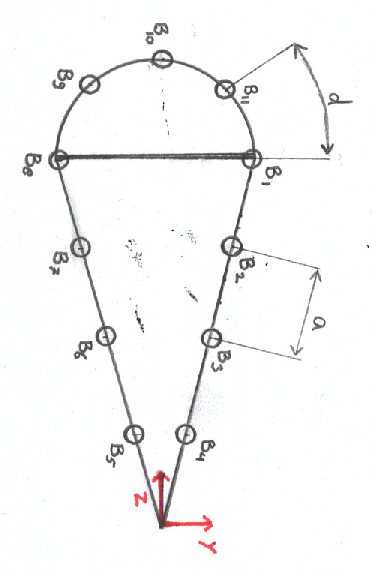
\includegraphics[width=6cm,angle=90]{Images/boom.pdf}
    \caption{Structural boom idealisation of the aileron structure}
    \label{fig:boom}
\end{figure}

\subsubsection{Moment of inertia}
\label{subsubsec:MoI}
The first and second moment of Inertia's around the x- and z-axes are calculated. This is done by taking the Steiner term for each boom \cite{the_book}. The formulas used for this are the following \eqautoref{MoI_xx}, \eqautoref{MoI_yy} and \eqautoref{MoI_zz}:
\begin{equation}
\label{MoI_xx}
    I_{x x}=\sum_{i=1}^{n} y_{i}^{2} B_{x_{i}}
\end{equation}

\begin{equation}
\label{MoI_zz}
    I_{z z}=\sum_{i=1}^{n} y_{i}^{2} B_{z_{i}}
\end{equation}

\subsubsection{Load cases}

There are three load cases considered for the concerning load scenario. These include all the loads acting on the aileron.
Firstly there is the aileron deformation due to the wing-flex of the main wing. Secondly, the aerodynamic load is considered, which is distributed over the aileron surface. Finally there is the discrete load $P$ acting on actuator $II$. All of these loads introduce reaction forces in hinges 1, 2 and 3. A more elaborate description and analysis is given in \autoref{subsec:load_decomposition}.

\subsubsection{Shear}
Shear flow experienced by the structure is caused by shear loads and torques. In this numerical model the shear flow distribution in the skin is calculated separately for external shear forces and external torques. This is done for each load case. Consequently the total shear flow distribution is determined by adding up the shear flow values. Knowing these values, the rate of twist around the x-axis can be calculated. This rate of twist is then numerically integrated over the span of the aileron to come to the total twist of the structure. For this, Gauss quadrature integration is used.
As is mentioned in \autoref{subsubsec:boom}, shear flows only through the skin.

\subsubsection{Normal stress}
Normal stresses are solely caused by the bending moment. As stated in \autoref{subsec:assumptions_numerical}, the numerical model only takes into account bending moment around the z-axis. The bending around x- and y-axis are neglected.
The normal stresses in each boom are determined from the bending moments caused by all three load cases. Then these are added up and this results in the total normal stress distribution in the structure.

\subsection{Flow chart}
The method of the simulation is also made visible with a flow chart (\autoref{flowchart}), in which the same chronological order (of the method) can be found. By following the numbers in the beginning of every square, it is clear that from the geometric properties first some necessary values are calculated (centroid, idealisation, moment of inertia). Afterwards the three load cases are analysed separately. Starting with the stresses induced by the wing deformation. Because this loading was not given it needs to be obtained in the opposite direction. From displacement to moment to stresses. To do this a linear system of equations and some boundary conditions are used.\\

\noindent For the two other load cases some extra inputs are needed, namely the loading itself. Despite the fact that these loads are solved in two different cases, their way of solving is the same. Namely analysing the load, solve for the reaction forces and the different internal loads and extracting the stresses from these internal loads.\\

\noindent All these elements are then combined together to get the ultimate load case from which the maximum stresses, angle of twist and deformations can be obtained.


\label{subsec:Flow_chart}
\begin{figure}[H]
    \centering
    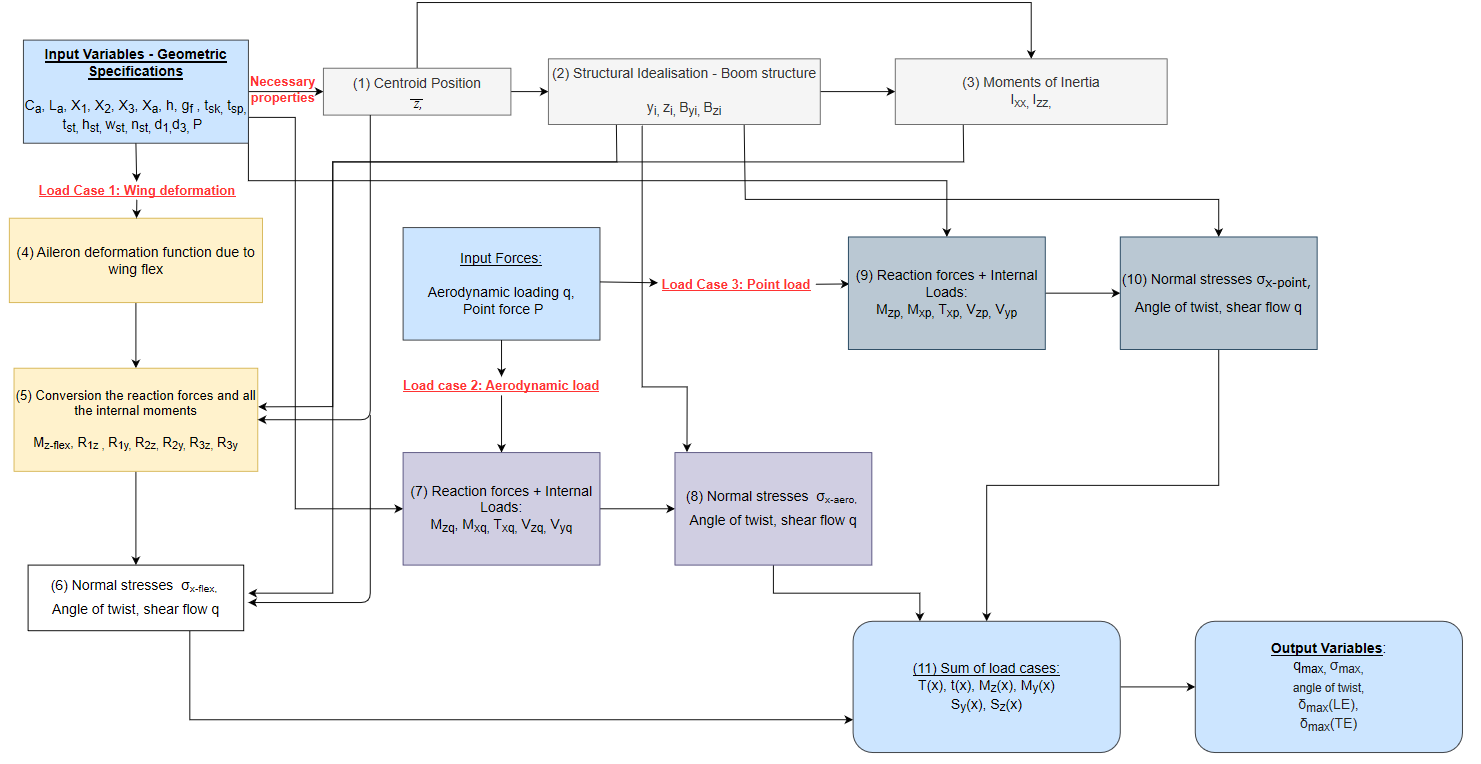
\includegraphics[width=23cm, angle=90]{Images/Flowchart3.PNG}
    \caption{Flowchart as illustration of the working principle of the simulation }
    \label{flowchart}
\end{figure}



















